\documentclass[tikz,border=5pt]{standalone}
\usepackage{amsmath}
\usepackage[T1]{fontenc}
\usetikzlibrary{calc}
\definecolor{region}{RGB}{96,115,182}
\definecolor{bounda}{RGB}{26,77,145}
\definecolor{boundb}{RGB}{181,70,65}
\definecolor{boundc}{RGB}{42,130,106}
\begin{document}

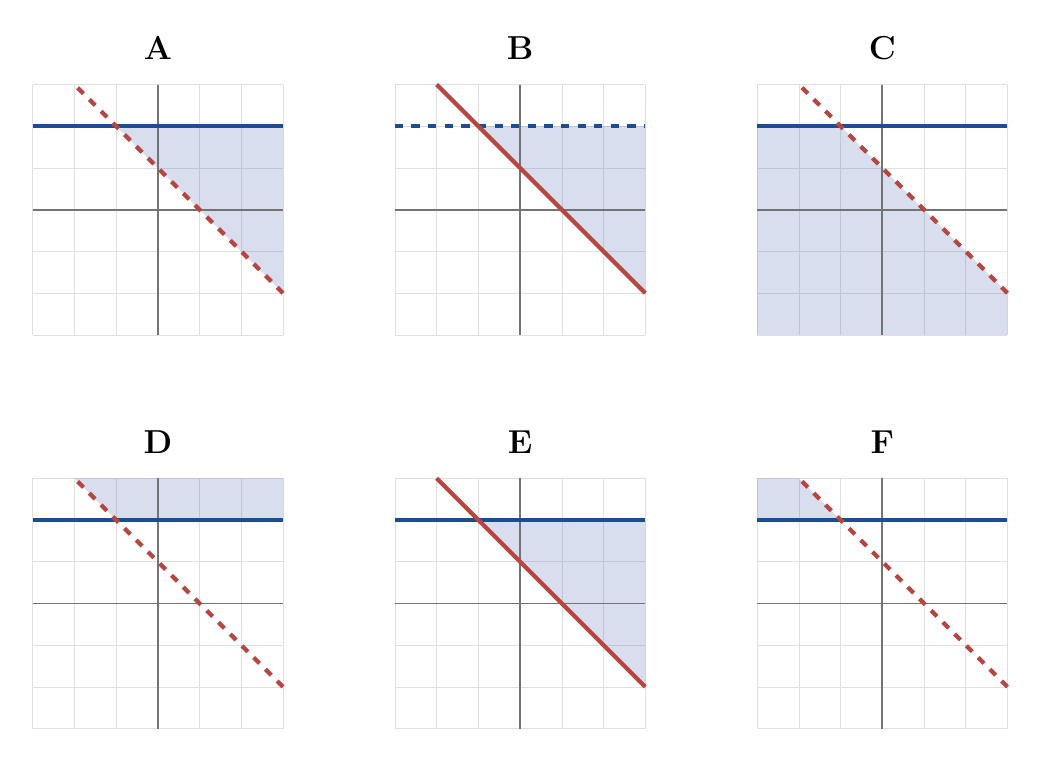
\begin{tikzpicture}
\begin{scope}[shift={(0.0,0.0)}]
\begin{scope}[scale=0.53]
\clip (-3.12,-3.12) rectangle (3.15,3.15);
\draw[step=1,gray!25,very thin] (-3,-3) grid (3,3);
\fill[region,opacity=.24] (3,-2) -- (3,2) -- (-1,2) -- cycle;
\draw[black!55,line width=.65pt] (0,-3) -- (0,3);
\draw[black!55,line width=.65pt] (-3,0) -- (3,0);
\draw[bounda,line width=1.55pt,solid] (-3,2) -- (3,2);
\draw[boundb,line width=1.55pt,dashed] (3,-2) -- (-2,3);
\end{scope}
\node[font=\bfseries\large] at (0,2.05) {A};
\end{scope}
\begin{scope}[shift={(4.6,0.0)}]
\begin{scope}[scale=0.53]
\clip (-3.12,-3.12) rectangle (3.15,3.15);
\draw[step=1,gray!25,very thin] (-3,-3) grid (3,3);
\fill[region,opacity=.24] (3,-2) -- (3,2) -- (-1,2) -- cycle;
\draw[black!55,line width=.65pt] (0,-3) -- (0,3);
\draw[black!55,line width=.65pt] (-3,0) -- (3,0);
\draw[bounda,line width=1.55pt,dashed] (-3,2) -- (3,2);
\draw[boundb,line width=1.55pt,solid] (3,-2) -- (-2,3);
\end{scope}
\node[font=\bfseries\large] at (0,2.05) {B};
\end{scope}
\begin{scope}[shift={(9.2,0.0)}]
\begin{scope}[scale=0.53]
\clip (-3.12,-3.12) rectangle (3.15,3.15);
\draw[step=1,gray!25,very thin] (-3,-3) grid (3,3);
\fill[region,opacity=.24] (3,-2) -- (-1,2) -- (-3,2) -- (-3,-3) -- (3,-3) -- cycle;
\draw[black!55,line width=.65pt] (0,-3) -- (0,3);
\draw[black!55,line width=.65pt] (-3,0) -- (3,0);
\draw[bounda,line width=1.55pt,solid] (-3,2) -- (3,2);
\draw[boundb,line width=1.55pt,dashed] (3,-2) -- (-2,3);
\end{scope}
\node[font=\bfseries\large] at (0,2.05) {C};
\end{scope}
\begin{scope}[shift={(0.0,-5.0)}]
\begin{scope}[scale=0.53]
\clip (-3.12,-3.12) rectangle (3.15,3.15);
\draw[step=1,gray!25,very thin] (-3,-3) grid (3,3);
\fill[region,opacity=.24] (3,3) -- (-2,3) -- (-1,2) -- (3,2) -- cycle;
\draw[black!55,line width=.65pt] (0,-3) -- (0,3);
\draw[black!55,line width=.65pt] (-3,0) -- (3,0);
\draw[bounda,line width=1.55pt,solid] (-3,2) -- (3,2);
\draw[boundb,line width=1.55pt,dashed] (3,-2) -- (-2,3);
\end{scope}
\node[font=\bfseries\large] at (0,2.05) {D};
\end{scope}
\begin{scope}[shift={(4.6,-5.0)}]
\begin{scope}[scale=0.53]
\clip (-3.12,-3.12) rectangle (3.15,3.15);
\draw[step=1,gray!25,very thin] (-3,-3) grid (3,3);
\fill[region,opacity=.24] (3,-2) -- (3,2) -- (-1,2) -- cycle;
\draw[black!55,line width=.65pt] (0,-3) -- (0,3);
\draw[black!55,line width=.65pt] (-3,0) -- (3,0);
\draw[bounda,line width=1.55pt,solid] (-3,2) -- (3,2);
\draw[boundb,line width=1.55pt,solid] (3,-2) -- (-2,3);
\end{scope}
\node[font=\bfseries\large] at (0,2.05) {E};
\end{scope}
\begin{scope}[shift={(9.2,-5.0)}]
\begin{scope}[scale=0.53]
\clip (-3.12,-3.12) rectangle (3.15,3.15);
\draw[step=1,gray!25,very thin] (-3,-3) grid (3,3);
\fill[region,opacity=.24] (-2,3) -- (-3,3) -- (-3,2) -- (-1,2) -- cycle;
\draw[black!55,line width=.65pt] (0,-3) -- (0,3);
\draw[black!55,line width=.65pt] (-3,0) -- (3,0);
\draw[bounda,line width=1.55pt,solid] (-3,2) -- (3,2);
\draw[boundb,line width=1.55pt,dashed] (3,-2) -- (-2,3);
\end{scope}
\node[font=\bfseries\large] at (0,2.05) {F};
\end{scope}
\end{tikzpicture}
\end{document}
